\documentclass[12pt, titlepage]{article}

\usepackage{booktabs}
\usepackage{tabularx}
\usepackage{hyperref}
\usepackage{graphicx}
\usepackage{enumerate}
\hypersetup{
    colorlinks,
    citecolor=black,
    filecolor=black,
    linkcolor=red,
    urlcolor=blue
}
\usepackage[round]{natbib}

\title{SE 3XA3: Software Requirements Specification\\Jumbled Words}

\author{Team 08, Shunbill Jumble
	\\Shesan Balachandran, balacs1
	\\Bill Nguyen, nguyew3
	\\Muneeb Arshad, arsham14
}

\date{\today}

%\input{../Comments}

\begin{document}
	

\maketitle

\pagenumbering{roman}
\tableofcontents
\listoftables
\listoffigures

\newpage
\begin{table}[bp]
\caption{\bf Revision History}
\begin{tabularx}{\textwidth}{p{3cm}p{2cm}X}
\toprule {\bf Date} & {\bf Version} & {\bf Notes}\\
\midrule
Feb 11 2021 & 0.0 & Initial Draft\\
\bottomrule
\end{tabularx}
\end{table}

\clearpage



\pagenumbering{arabic}

This document describes the requirements for Jumbled Words. The template for the Software
Requirements Specification (SRS) is a subset of the Volere
template ~\citep{RobertsonAndRobertson2012}. This document will highlight the stakeholders, functional and non-functional requirements, and the constraints presented in the completion of the product.

\section{Project Drivers}

\subsection{The Purpose of the Project}

The purpose of this project is to improve on the desktop version of the product/game “Jumbled Words” in order to deliver a more complete version of the product. This more complete version of the product will include many new features such as new game modes such as a practice/learning mode where the user can decipher new words with an unlimited amount of guesses in order to decipher new words in a less competitive environment and also a new timer mode where there will be a timer for a set amount of time and the user has to decipher as many words as possible in the limited time. Other features include adding different difficulty levels where each difficulty will be based on the length of the word and a limited number of guesses, adding a leaderboard in order to develop a more competitive aspect to the game and improving the limited amount words that are already in the product by integrating a word library in order to store more words that will be useful to make this product more educational and enjoyable. The code of the product will also be very maintainable, modular, well documented and tested, which will allow any potential future developers to modify, reuse and understand the code.

\subsection{The Stakeholders}

\subsubsection{The Client}

The clients for the product are the team members of Group-8 who are the final testers of the product before it is made public. Other clients include the teaching staff of the Software Engineering 3XA3 course that will be involved in the development process of the project.

\subsubsection{The Customers}

The customers for the product are the students and the general public who enjoy puzzle games and are interested in enhancing their vocabulary and spelling skills. Customers of this product also include teachers and instructors who are looking for an educational game for their students.

\subsubsection{Other Stakeholders}

Other stakeholders include potential developers who wish to improve and add features to this product.

\subsection{Mandated Constraints}

Product Constraints\\
\\
To use the product, the users will require a pc that is running either Windows or macOS. The product will require text input and a cursor input, so a keyboard and a mouse will be required to play and a controller is not supported by this product.\\
\\
User Constraints\\
\\
The users need to have basic knowledge of navigating the product with a mouse and need to know English to navigate as well as play our product.\\
\\
Time Constraints\\
\\
The product must be completed in a time frame of 3 months. The initial version must be released in the month of April 2021.\\
\\
Budget Constraints\\
\\
The budget is restricted to \$0. This means the product must be built using open source technologies and custom tools and no licensed product can be used in the development of this product.


\subsection{Naming Conventions and Terminology}

GUI - Graphical User Interface\\
\\
macOS - GUI based operating system used in Macintosh series of personal computers\\
\\
Windows - Most commonly used GUI based operating system in personal computers\\
\\
Group-08 - The team of product developers\\

\subsection{Relevant Facts and Assumptions}

Facts
\begin{enumerate}
	\item The product is developed in python.
	\item The original product has no documentation for the code.
	\item Tkinter library is used for the UI of the product. 
	\item The product will run only on desktops.
\end{enumerate}

\noindent Assumptions
\begin{enumerate}
	\item The user has the necessary knowledge to be able to interact with the hardware required to use the product.
	\item The user has basic proficiency in the English language.
	\item The personal computer used is powerful enough to run the product.
\end{enumerate}

\section{Functional Requirements}

\subsection{The Scope of the Work and the Product}

The software product in this document is a single-player Jumbled Word game with a GUI designed for desktop.  The project will include deliverables such as design documents, requirement specification and testing, with a development time span of 4 months and zero cost. The goal of this product is to make educational games more interesting and add another layer to the learning aspect and provide educational value in the gaming market. 
The objective of this product is to provide a platform to provide a fun and interactive solution to help others learn how to spell through various game modes and high scores and leaderboards as an incentive to do their best. A progressive difficulty setting is also added as a feature to challenge the users as they get better and better at spelling. The benefit of this product is to allow users to enhance vocabulary and spelling skills. 

\subsubsection{The Context of the Work}

\begin{figure}[h]
	\centering
	\includegraphics[width=\textwidth]{context_of_work}
	\caption{Context Diagram}
\end{figure}

\subsubsection{Work Partitioning}

% Begin Section
\begin{table}[h]
	\begin{center}
		\begin{tabular}{|p{0.1\textwidth}|p{0.3\textwidth}|p{0.6\textwidth}|}
			\hline
			Number & Event Name & Input and Output\\ 
			\hline
			BE1 & The user enters a new username & Username Updated(out) \\
			\hline
			BE2 & The user selects the desired game mode & Game Input(out), Game Mode Updated(in), Game State Updated(in) \\ 
			\hline
			BE3 & The user selects desired difficulty level & Difficulty Level Updated(in), Game State Updated(in)\\
			\hline
			BE4 & The user quits the current game & User Game Input(in), Game State Updated(out)\\
			\hline
			BE5 & The user guesses a word & User Game Input(in), Game State Updated(out)\\
			\hline
			BE6 & The user selects the desired category & Category Updated(in), Game State Updated(in) \\
			\hline
			BE7 & The user access leaderboard & Leaderboard Updated(in) \\
			\hline
		\end{tabular}
	\end{center}
	\caption{Business Events}
	\label{tab:my_label}
\end{table}

\newpage

\subsubsection{Individual Product Use Cases}

% Begin Section
\begin{table}[h]
	\begin{center}
		\begin{tabular}{|p{0.1\textwidth}|p{0.3\textwidth}|p{0.6\textwidth}|}
			\hline
			Number & Usecase & Summary\\ 
			\hline
			UC1 & Enter username & The user enters their desired username, and the system saves the username to the local User Database \\
			\hline
			UC2 & Select game mode & The user selects learning mode or timed mode. \\ 
			\hline
			UC3 & Select difficult level & The user selects the difficulty level from easy, medium or hard. \\
			\hline
			UC4 & Quit game & The user clicks on the back button to quit the current game. \\
			\hline
			UC5 & Guess word & The user is able to successfully guess the word from the given jumbled letters\\
			\hline
			UC6 & Select category & The user selects the word category. \\
			\hline
			UC7 & Access leaderboard  & The user clicks on the leaderboard button to view the leaderboard \\
			\hline
		\end{tabular}
	\end{center}
	\caption{Usecase}
	\label{tab:my_label}
\end{table}

\begin{figure}[]
	\centering
	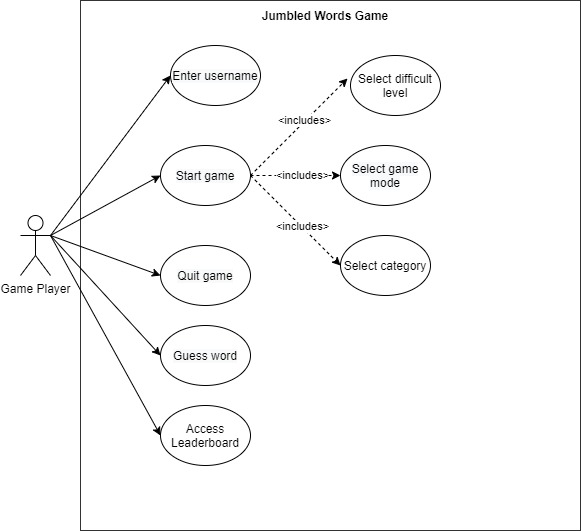
\includegraphics[width=\textwidth]{usecase_2}
	\caption{Use Case Diagram}
\end{figure}

\clearpage

\subsection{Functional Requirements}

\begin{enumerate}[{FR}1.]
	\item The product shall allow the user to enter a username.
	{\newline \emph{Rationale}:  To ensure the user has a name to record scores and to be able to play the product. 
	\newline \textbf{Fit Criterion}: The user is able to input a name, the name shall be the name entered by the user and once the name is entered the user shall proceed to the next part.} 
	
	\item The product shall allow the user to select the desired game mode.
	{\newline \emph{Rationale}:  The user needs to select the desired game mode, or else the user cannot play the product.
	\newline \textbf{Fit Criterion}: The game mode will correspond to the game mode selected by the user and will proceed to the next part.}
	
	\item The product shall allow the user to select the desired difficulty level from easy, medium or high.
	{\newline \emph{Rationale}:  The user needs to select the difficulty level, or else the user cannot play the product.
	\newline \textbf{Fit Criterion}: The difficulty level will correspond to the difficulty level selected by the user and will proceed to the next part.}
	
	\item The product shall allow the user to select the desired category.
	{\newline \emph{Rationale}:  The user needs to select the desired category, or else the user cannot play the product.
	\newline \textbf{Fit Criterion}: The category will correspond to the category selected by the user and will proceed to the next part.}
	
	\item The username and points shall be displayed on the leaderboard after the game ends.
	{\newline \emph{Rationale}: The user should be able to track achievements and high scores.
	\newline \textbf{Fit Criterion}:The product will record the score of the user once the game is over and add it to the leaderboard if the score is greater than any of the 10 previous scores, with the 10th score being removed from the leaderboard.}
	
	\item The product shall provide notification to the user if the guess is invalid/incorrect.
	{\newline \emph{Rationale}: The user needs some method to know that their guess is invalid/incorrect.
	\newline \textbf{Fit Criterion}: Guess an invalid/incorrect word and a notification will appear indicating the guess is invalid/incorrect.}
	
	\item The product shall give the user 5 points and a new word to guess when the user guesses/deciphers a word correctly.
	{\newline \emph{Rationale}: Part of the product/game is guessing/deciphering the word correctly, so when the user guesses correctly the user should be rewarded and given another word.
	\newline \textbf{Fit Criterion}:  Guess a word correctly and 5 points will be given to the user and a new word will appear for the user to guess.}
	
	\item The product must allow the user to quit the game at any given time.
	{\newline \emph{Rationale}: To ensure the game is exited successfully without the user being forced to complete the game.
	\newline \textbf{Fit Criterion}:The product must allow the user to click the back button during the game and then click the quit game button on the main menu to successfully exit the game. }
	
	\item The system shall display the current game state of the user.
	{\newline \emph{Rationale}: The user needs to have the ability to show the current game state or else, the product will be unplayable and inconsistent.
	\newline \textbf{Fit Criterion}: The game state that is displayed must match the current game state. }
	
	\item For the timed game mode after the time has run out a notification must appear indicating the score of the user and options to start a new game or return to the main menu.
	{\newline \emph{Rationale}: Once the game is finished the user needs to be able to return to the main menu or start a new game.
	\newline \textbf{Fit Criterion}: Once the timer has run out, the score of the user must be recorded and added to the leaderboard and a notification will appear indicating to start a new or return to the main menu. }
	
	\item The product must allow the user to access the leaderboard.
	{\newline \emph{Rationale}: The leaderboard is an important feature of the product, allowing the users to compare scores, gives the users motivation to improve their scores, and gives a competitive aspect to the product.
	{\newline \textbf{Fit Criterion}: The product must allow the user to access the leaderboard and the leaderboard must display the highest scores from highest to lowest. The leaderboard shall only display usernames with top 10 scores.
	
	\item The Product shall have the main menu screen for standby.
	{\newline \emph{Rationale}: The main menu screen, gives the user the option to start the game when they want to.
	\newline \textbf{Fit Criterion}:The product must display the main menu screen, once the user opens the product.}

\end{enumerate}

\section{Non-functional Requirements}

\subsection{Look and Feel Requirements}

\begin{enumerate}[{NFR}1.]
	\item The product should have an aesthetically appealing GUI. \newline \emph{Rationale}:  Making sure the users will have a pleasant experience while playing the product.\newline \textbf{Fit Criterion}: More than 75\% of users like the icons, fonts and colours used in the product.
\end{enumerate}

\subsection{Usability and Humanity Requirements}

\begin{enumerate}[{NFR}2.]
	\item The product shall have a user-friendly interface.\newline \emph{Rationale}: Making sure the product is easy to use.
		\newline \textbf{Fit Criterion}:  A new user should be able to navigate through all the paths available in the interface without assistance.
\end{enumerate}

\subsection{Performance Requirements}
\begin{enumerate}[{NFR}3.]
	\item The product will have a fast response time for any user operation on the GUI.\newline \emph{Rationale}:  Making sure the product is fast and responsive and will not frustrate the user by making them wait.\newline \textbf{Fit Criterion}: All the user clicks and keyboard inputs possible will be tested multiple times and all of them must respond within 2 seconds on screen. 
\end{enumerate}

\subsection{Operational and Environmental Requirements}

\begin{enumerate}[{NFR4}.1]
	\item The product will be tested on multiple devices matching this version to test the operating system supportability and the product should work as usual.
	\newline \emph{Rationale}:  Making sure the product must be supported on popular operating systems.
	 them wait.\newline \textbf{Fit Criterion}: The product will be tested on multiple devices matching this version to test the operating system supportability and the product should work as usual.
	 
	 \item The product must be able to run on a minimum 1Gb of ram and 1 Gb of disk space. 	 
	 \newline \emph{Rationale}:  Making sure the product performance depends on the hardware resources but given a minimum, it must perform optimally.
	 them wait.\newline \textbf{Fit Criterion}: The product will be tested on multiple devices matching these hardware requirements and the product must work as usual.	
\end{enumerate}

\subsection{Maintainability and Support Requirements}

\begin{enumerate}[{NFR5}.1]
	\item  The product must include code documentation to support future developments and fixes. 
	\newline \emph{Rationale}:  Making sure the product has enough resources for maintainability.
	them wait.\newline \textbf{Fit Criterion}: All developers should agree that the documentation provided is enough to get started with potential changes.
	
	\item The product will be updated frequently with bug fixes, user requests and new features. 
	\newline \emph{Rationale}:  Making sure the product has new content to keep the users engaged and coming back.
	them wait.\newline \textbf{Fit Criterion}: The developers have a defined schedule to support and help out with the frequent updates.
\end{enumerate}

\subsection{Security Requirements}

\begin{enumerate}[{NFR6}.1]
	\item  The user information such as the user name and their high scores should be stored securely. 
	\newline \emph{Rationale}: Making sure the user data used is safe and not easily accessible.
	them wait.\newline \textbf{Fit Criterion}: The user data must be encrypted before it is stored in the database and the database must then only store encrypted content.
	
	\item One user cannot access or modify the data of another user without credentials. 
	\newline \emph{Rationale}: Making sure the users only have access to their data and nobody else.
	them wait.\newline \textbf{Fit Criterion}: The product shall only update data for the user that is currently using it so all other user information should not be modified in any shape or form during this session.
	
	\item The product will prevent a new user to register under a pre-existing username. 
	\newline \emph{Rationale}: Making sure there are unique users so user data will not get overlapped or lost.
	them wait.\newline \textbf{Fit Criterion}: All attempts to create such usernames will result in a failure.
\end{enumerate}

\subsection{Cultural Requirements}

\begin{enumerate}[{NFR}7.]
	\item  The product must not use icons, texts or symbols that are discriminatory against any background. 
	\newline \emph{Rationale}: Making sure the product is culturally acceptable and no one is discriminated against while playing the game.
	them wait.\newline \textbf{Fit Criterion}: A test group of people from various cultures and ethnicities should accept all the details in the product as in confirming there is no cultural discrimination.
\end{enumerate}

\subsection{Legal Requirements}

\begin{enumerate}[{NFR8}.1]
	\item  The product developed should not conflict with any licensing.
	\newline \emph{Rationale}: Making sure the product does not conflict with licensing issues.
	them wait.\newline \textbf{Fit Criterion}: The product must satisfy the licensing attached to the original product which is none and it is completely free of use.
	
	\item The product must not include copyrighted content like copyrighted music, icons or images. 
	\newline \emph{Rationale}: Making sure the product does not use content without authorization.
	them wait.\newline \textbf{Fit Criterion}: The product must use only free of use material or custom made content.
\end{enumerate}

\subsection{Health and Safety Requirements}

\begin{enumerate}[{NFR9}.1]
	\item  The product must not track any of the user data like personal name or email but only their username and their scores.
	\newline \emph{Rationale}: Making sure the product does not put the user’s personal information at risk.
	them wait.\newline \textbf{Fit Criterion}: All the data stored in the database could be checked at any point to confirm this requirement.
	
	\item The product must not display any flashing lights or patterns that are sensitive to those with epilepsy. 
	\newline \emph{Rationale}:Making sure the product does not affect people with epilepsy.
	them wait.\newline \textbf{Fit Criterion}: A test group of users with epilepsy must be able to successfully use the product for 1 hour without any health issues.
\end{enumerate}

\section{Project Issues}

\subsection{Open Issues}

No open issues have been identified.

\subsection{Off-the-Shelf Solutions}

Since the product is a recreation/improvement of an existing Jumbled Words game, a basic product already exists. However, the base product offers limited features and functionalities and misses the ‘game’ aspect of the product. The basic functionality of guessing jumbled words is there but it is still quite far from a functional product that can be distributed to users and has brought in enough audience to have to maintain and support the software.\\
\\
The original jumbled words game can be found here: \href{https://code-projects.org/jumbled-words-quiz-in-python-with-source-code/}{Link}

\subsection{New Problems}

As for technical problems, a brand new backend to integrate all the new features together arises. From unit level to system-level testing needs to be implemented from the ground up for existing code, as well as new ones. As for the entertainment aspect, the product is projected for a wide range of audiences, from children to adults. The product must be easy enough for children to start playing and enjoying the game but also challenging and fun for the adults to continue playing and come back to. 

\subsection{Tasks}

All tasks that need to be accomplished are covered in the Gantt Charts provided in the project planning, which includes the allocation of time for specific tasks as well as the deadlines.\\
\\
The Gantt charts can be found here: \href{https://gitlab.cas.mcmaster.ca/balacs1/se3xa3-project/-/tree/master/ProjectSchedule}{Link}

\subsection{Migration to the New Product}

Due to an overhaul of the backend, many of the system-level code must be redone. However individual components will be carried over. These individual components will have dedicated testing as none was provided initially, with maintainability in mind, automated and regression testing will also be utilized. An executable version will also be available to be downloaded, unlike the current product that is executed through the command line.

\subsection{Risks}

Testing is a risk that must be assessed. Because the base product has no testing involved, testing functions must be developed from the ground up. This also means that any necessary changes required for the original code after testing must be done on top of the new features that the team will be working on. If the base code has significant issues, the limited time for the development of the new product will be of concern to plan ahead.

\subsection{Costs}

There is no cost involved in the development of this product as the budget is \$0.

\subsection{User Documentation and Training}

The product will be developed with ease of learning and usability in mind as mentioned in the requirements above. Hence separate user documentation nor training will be necessary. Although a sample playthrough will be provided as guidance and an introduction to the application.

\subsection{Waiting Room}

There are no additional requirements for future releases yet.

\subsection{Ideas for Solutions}

\begin{enumerate}
	\item The development will leverage tools and technologies already used in the base product, like Python, and Tkinter for the front end.	
	\item The local database should be implemented as a local JSON file system, which includes the user data, high scores and the word library. 
\end{enumerate}

\section{Appendix}

\subsection{Symbolic Parameters}

N/A

\newpage

\bibliographystyle{plainnat}

\bibliography{SRS}

\newpage


\end{document}